\documentclass[12pt]{report}

\usepackage[a4paper,
			inner = 35mm,
			outer = 25mm,
			top = 25mm,
			bottom = 25mm]{geometry}
\usepackage{lmodern}
\usepackage[magyar]{babel}
\usepackage[utf8]{inputenc}
\usepackage[T1]{fontenc}
\usepackage[hidelinks]{hyperref}
\usepackage{graphicx}
\usepackage{amssymb}
\usepackage{setspace}
\usepackage[nottoc,numbib]{tocbibind}
\usepackage{amsthm}
\usepackage{minted}
\usepackage{mdframed}
\usepackage{etoolbox}



% \setcounter{secnumdepth}{3}
\onehalfspacing

\newtheorem{mydef}{Definició}
\newtheorem{mytetel}{Tétel}
\newtheorem{mylemma}{Lemma}

\BeforeBeginEnvironment{minted}{\begin{mdframed}[backgroundcolor=bg, hidealllines=true]}
\AfterEndEnvironment{minted}{\end{mdframed}}

\newcommand{\cmd}[1]{\colorbox{gray!10}{\strut #1}}

\definecolor{bg}{rgb}{0.95,0.95,0.95}
\newminted[mintedJson]{js}{breaklines, breaksymbolleft=\quad}
\newminted[mintedBash]{bash}{breaklines, breaksymbolleft=\quad}



\begin{document}

\begin{titlepage}
	\begin{center}
		\vspace*{1cm}
		
		\textbf{\LARGE 
			Forgalom igény tudatos hálózat tervezés minimális torlódással és úthosszal
		}
	
	
		\vspace{0.5cm}
	
		\textbf{\normalsize Tudáskezelő rendszerek III. labor összefoglaló}
		
		\vfill
		
		\Large Szecsődi Imre
		
		\vspace{2.8cm}
		
		\the\year
		
	\end{center}
\end{titlepage}

\tableofcontents
	
\chapter{Bevezetés}


\section{Labor célja}

A labor célja a korábban már bemutatott cikk\cite{avin_demand-aware_nodate} hálózat építése.
Az eredeti cikkben a fák építésére az Egofa algoritmus volt használva, a labor keretén belül azt a felvetést vizsgáltam meg, hogy lehet-e jobb algoritmust találni fa építésre, mint az Egofa. 
A különböző módszerek az eredetihez hasonlóan véletlenszerűen generált gráfokra vannak tesztelve. 
Az új módosított algoritmusok eredménye az eredetivel voltak összehasonlítva.

\section{Laborban megvalósított munka}

A labor ideje alatt a már elkészült keretrendszer adta az alapot, ami segítségével tesztelhető a szerzők által felvázolt és három saját fejlesztésű algoritmus is.
A keretrendszer Python \cite{noauthor_python_nodate} nyelven íródott.
Egy véletlen gráfok generálására a NetworkX külső csomag volt használva\cite{noauthor_networkx_nodate}.
Az adatok elemzése pedig RapidMiner-ben történt\cite{noauthor_lightning_nodate}.

\chapter{Modell}

\section{Az új algoritmusok}

\subsection{Egobalance}

Az első algoritmus majdnem teljes mértékben megegyezik az eredetivel.
A cikk szerzői az Egofa algoritmus vázlatos összefoglalásában használtak egy csere lépést.
A csere lépés lényege, hogy mikor megépítettük a fákat, azután ki kell iktatni a direkt kapcsolatokat a magas-magas csomópontok között.
Mikor a segítő nincs a fában, ott nincs semmi egyéb tenni valónk, mivel egy csere történik, és a csomópont gyerekei nem vándorolnak sehova.
Ezzel ellentétben, mikor a segítő pont is része a fának, akkor két lehetőségünk van, ha a segítő közelebb van a gyökérhez akkor töröljük a magas pontot, ha pedig a magas pont van feljebb, akkor a segítő átveszi a helyét, majd töröljük a magast.

A említett algoritmus egyik lényeges része, hogy mi történik a gyerekekkel, mivel vagy a segítő vagy a magas pont gyerekeit kell újra visszakapcsolni a fára.
Az eredeti implementációban a törölt csomópont szülőjére lett rákapcsolva a nehezebb gyerek, és a maradék fa pedig hasonló elven, addig hozta fel a nehezebb pontot még minden hiányzó belső csomópont nem lett kitöltve. Az Egobalance logaritmus a függő pontok újra elhelyezését az Egofára bízza, azaz újra elosztásra kerülnek.
Ezzel elméletben mindig arra törekszik a fa, hogy optimális legyen torlódásra nézve az új fa.
Lényegi különbség úthossznál jelentkezik az eredetivel szemben.

\subsection{Huffman fa}

A eddigi két algoritmus az Egofát használta, ami optimális torlódásra nézve, de mivel a hálózat nem csak torlódás szempontjából van vizsgálva ezért meg kell vizsgálni a másik aspektusát is az optimális úthosszt.
A Huffman kódolásnál használt fa tulajdonsága, hogy átlagosan rövidek legyenek a gyakoriságot tekintve.
A cl-Dan probléma is ezt a tényezőt használja, ezért kitűnően lehet használni ezt a fát a hálózat alapjának.
Egyetlen probléma a Huffman fával az, hogy a belső csomópontok nem tartalmaznak számunkra hasznos információt.
Ezért szükséges egy kiegészítő lépés, ami segítségével belső pontok is ki lesznek töltve hasznos információval, azaz esetünkben csomópontokkal, amik maguk is végpontok, mint a levelek.

Az algoritmus első része teljesen megegyezik a Huffman kódolással.
Rendezzük sorba növekedően a pontokat, és kettesével vonjuk össze őket, még nem kapunk egy teljes fát.
Egy kis kiegészítés itt, hogy hasonlóan mint az Egofáknál, a legfelső szinten \(n\) darab csúcsot tudunk a gyökérre kapcsolni, ami maga a forrás csomópont.
Az összes többi alacsonyabb pont pedig marad bináris.

A belső pontok kitöltése pedig a következő módon történik:
\begin{enumerate}
	\item A gyökér csomóponthoz kapcsolódó ágakon szedjük össze a leveleket
	\item Ezeket a leveleket sorfolytonosan kapcsoljuk rá ág gyökér csomópontjára, az előtt említett bináris módon
\end{enumerate}
 
Felmerülhet a kérdés, hogy miért nem a legnehezebb levél jön fel mindig?
Ez azért van, mert a Huffman kódolásnál megtörténik az az eset, hogy két csomópont összesített értéke megegyezik egy harmadikkal.
Ez olyan fát eredményez, ahol bal oldalon egy nehéz csomópont és jobb oldalon fában két könnyű csomópont szerepel.
A naiv megoldás esetén ez azt eredményezi, hogy az egy nehéz lesz a belső csomópont, és az ág ahonnan jött megüresedik.
A pont levelei nem fognak ágat változtatni, annak ellenére, hogy megüresedett az egyik feljebb, ezért hosszú egyenes utak jöhetnek létre.
Ennek kiküszöbölésére van a sorfolytonos algoritmus, ahol garantálni lehet, hogy fa egyik belső csomópontja sem marad kitöltetlen levél nélkül.

\subsection{Sorfolytonos fa}

Mint láthattuk korábban a Huffman fánál láttuk a levelek felfelé mozgatását sorfolytonosan, itt hasonló az elv.
Lényegi különbséggel, hogy itt még a Huffman kódolási algoritmust kihagyjuk, és egyenest sorfolytonosan rakjuk már eleve fel csomópontokat.
Ezzel mindig a legkisebb fákat kapjuk, de ez a torlódást egyáltalán nem veszi figyelembe.

\chapter{Megvalósítás}

\section{Keretrendszer}

A keretrendszer Python 3 nyelven íródott, és a Networkx külső csomag volt használva a véletlen gráfok generálására.
A példakód megtalálható futtatható hagyományos Python programként és Jupyter notebookban \cite{noauthor_jupyter_nodate}].  
Networkx csomag továbbá biztosít számunkra egy megjelenítési lehetőséget, amit a Jupyter notebookban tudunk legjobban kihasználni.



\section{Adatszerkezetek}

A modell alapját pár egyszerű alaptípus adja. Ezek rendre a következők:
\begin{itemize}
	\item \textbf{Vertex} - az általános gráf csúcspont
	\item \textbf{Node} - az \textit{Egófák} készítésekor használt csomópontok amik tartalmazzák a valószínűségét annak, hogy a forrás csomópont mekkora valószínűséggel fog kommunikálni a másik \textit{Node} csomóponttal
	\item \textbf{Edge} - az gráf csomópontjait reprezentáló él, ami \textit{Vertexet} vár paraméterként, és tárolja a valószínűséget, hasonlóan mint a \textit{Node}
	\item \textbf{Tree} - ami adja az alapját majd a útvonal tervezési sémának. A fának két fajtája lehet:
	\begin{itemize}
		\item \textbf{BinTree} - a kettő fokú fa
		\item \textbf{EgoTree} - a $\Delta$ fokú fa, ahol a gyökérnek legfeljebb $\Delta$ levele lehet, és a levelek pedig \textit{BinTree} típúsuak.
	\end{itemize}
	
\end{itemize}
	
\section{Modell}

A \textbf{Network} osztály valósítja meg az algoritmust, bemenete egy konfiguráció, kimenete egy útválasztási séma.
Ez mellett sok metaadatot is kiszámol a program amik között szerepel az átlag súlyozott úthossz és a torlódás.
A konfigurációban lehetőségünk van dinamikus delta fokszámot megadni, ezért metaadatok között szerepel a fokszám, amit az algoritmus használt számoláskor.
Az új hálózat létrehozásakor a csere lépéssorozat után, megváltozik a demand mátrix, ezért fontos, hogy a \(\Delta\) fokszámot ne haladjuk meg.
A metaadatok ezért tartalmazzák a delta fokszámot és a valós fokszámot, ami az algoritmus végeredménye lett.  
Ebből az adatból lehet következtetést levonni, hogy valóban megfelelő-e felső korlátja amit a szerzők adtak és lehet-e jobb felső korlátot adni. 

A bemeneti konfiguráció egy \textit{JSON} fájl, amit tartalmazhat több konfigurációt egyszerre.
Többféle módon lehet megadni konfigurációt attól függően milyen gráfot akarunk használni. 
Lehetőség van kézileg megadni a demand mátrixot vagy generálhatunk kétféle gráfot.
Véletlen gráfok amit tud generálni a program:
\begin{itemize}
	\item Erdős-Rényi gráf
	\item Barabási-Albert gráf
\end{itemize}

Egy minta konfiguráció, ami tartalmaz példát mind három esetre:

\begin{mintedJson}
{
  "config": [ {
	"graph": "erdos-renyi",
	"vertex_num": 11,
	"dan": null,
	"constant": 3
  }, {
	"graph": "barabasi-albert",
	"vertex_num": 11,
	"dan": 3,
	"m": 4
  }, {
	"graph": "manual",
	"vertex_num": null,
	"dan": 3,
	"demand": [
		[0, 3, 4, 1, 1, 1, 1],
		[3, 0, 2, 0, 1, 0, 4],
		[4, 2, 0, 2, 0, 0, 4],
		[1, 0, 2, 0, 3, 0, 0],
		[1, 1, 0, 3, 0, 0, 0],
		[1, 0, 0, 0, 0, 0, 3],
		[1, 4, 4, 0, 0, 3, 0]]	
	} ]
}
\end{mintedJson}

A konfigurációnak van három kötelező mezője, és a egy kiegészítő mező, attól függően, hogy melyik típusú gráfot választottuk. 

Kötelező mezők: 
\begin{enumerate}
	\item \textbf{graph} - a gráf típusa, három érték közül lehet választani:
	\begin{itemize}
		\item \textit{"erdos-renyi"} - Erdős-Rényi gráf 
		\item \textit{"barabasi-albert"} - Barabási-Albert gráf
		\item \textit{"manual"} - Kézzel megadott gráf
	\end{itemize}
	\item \textbf{vertex\_num} - A gráf csúcsainak száma. Ez nincs figyelembe véve kézzel adott gráf esetén, mivel meg van adva a demand mátrix és nem kell azt kigenerálni.
	\item \textbf{dan} - A Demand-Aware Network fokszámára ad megkötést. Értékek amit felvehet:
	\begin{itemize}
		\item \textit{null} - Alap beállítás szerint a cikkben ajánlott $12\rho$ fokszámot fogja használni
		\item \textit{12} - A megadott szám lesz a fokszám, példában most 12.
		\item \textit{"6d"} - A szám és egy "d" betűvel a végén hasonlóan működik mint az első eset, annyi különbséggel, hogy itt meg lehet adni, hogy mi legyen a $\rho$ szorzója, példa most $6\rho$
	\end{itemize}
\end{enumerate}

Konfiguráció függő mezők:
\begin{itemize}
	\item \textbf{constant} - \textit{Erdő-Rényi} gráf esetén a modell vár egy \(p\) valószínűséget ami annak a valószínűsége, hogy egy él be legyen húzva az új pontba, és ez független minden a korábban behúzott élektől. 
	A ritka mátrix eléréséhez a következő formulát használja a generáló algoritmus:  \[p = constant \cdot \frac{1}{vertex\_num}\]
	\item \textbf{m} - \textit{Barabási-Albert} gráf esetén a modell vár egy \(m\) számot, ami azt adja meg, hány olyan gráf ponthoz kell csatlakozzon az új, ami már eddig benne van a gráfban. 
	\item \textbf{demand} -  \textit{kézzel megadott} gráf esetén direkt módon megadható a mátrix, aminek a formája listák listája. 
	Figyeljünk arra, hogy négyzetes lehet csak a demand mátrix!
\end{itemize}

\section{Kimenet}

Az program kimenete, az algoritmus által kiszámolt metrikák, átlag súlyozott úthossz és torlódás. 
Ha a rajzolás opció be van kapcsolva, akkor a kiindulási hálózat, az egófák és az új hálózat választási séma ki lesz rajzolva.

\begin{figure}[h]
	\begin{center}
		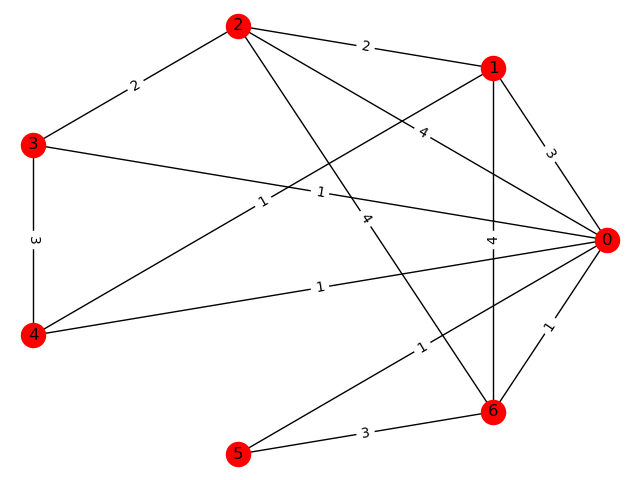
\includegraphics[width=0.49\linewidth]{pictures/starting_network.png}
		\caption{Kiindulási hálózat}
		\label{starting-network}
	\end{center}
\end{figure}

A \ref{starting-network} ábrán látható a bemeneti hálózat, aminek a demand mátrixa már a korábban fel lett írva. Az algoritmus ezek után a cl-DAN algoritmust használva, először elkészíti az egófákat \ref{ego-trees} ábra, majd végül az új hálózat választási sémát ami a \ref{routing-scheme} ábrán látható.

\begin{figure}[h]
	\begin{center}
		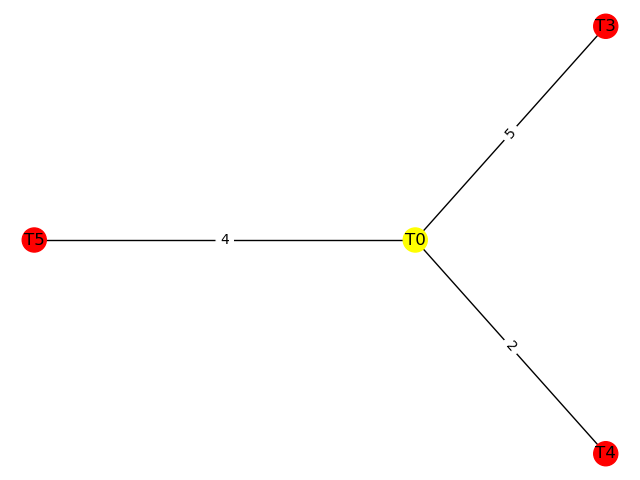
\includegraphics[width=0.40\linewidth]{pictures/egotree1.png}
		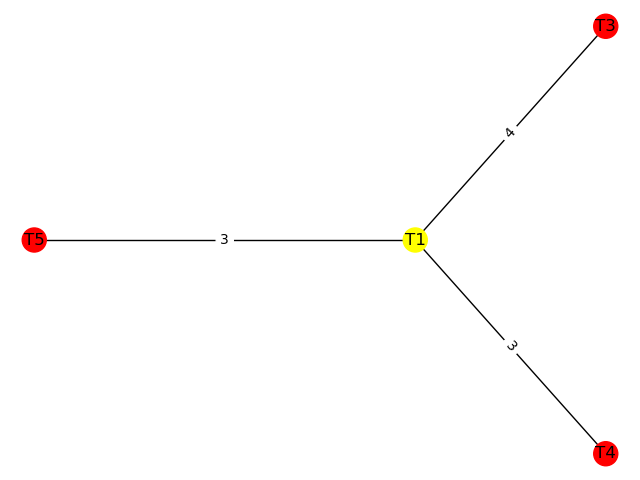
\includegraphics[width=0.40\linewidth]{pictures/egotree2.png}
		%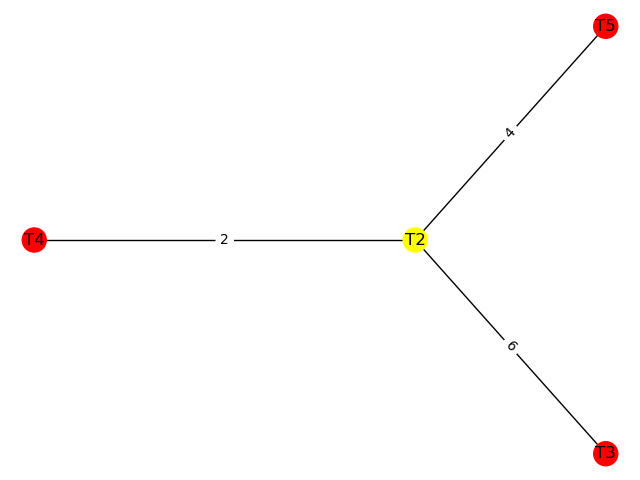
\includegraphics[width=0.40\linewidth]{pictures/egotree3.png}
		%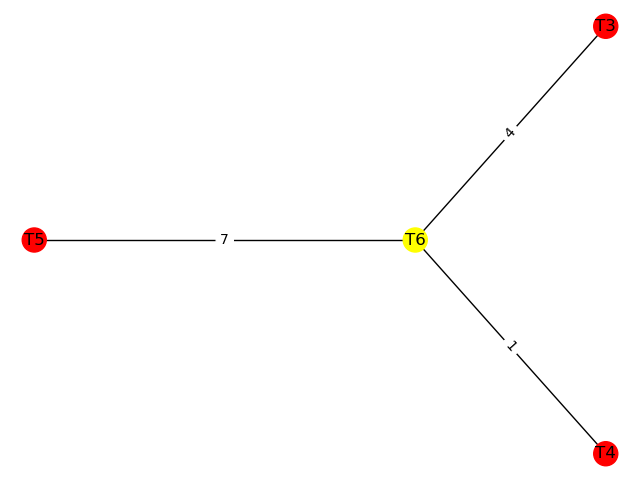
\includegraphics[width=0.40\linewidth]{pictures/egotree4.png}
		\caption{Egófák}
		\label{ego-trees}
	\end{center}
\end{figure}

A \ref{routing-scheme} ábrán látható gráfon pár extra információ megfigyelhető. 
Pirosra vannak festve a magas fokszámú csúcsok és zöldre az alacsony fokszámúak.
Az algoritmus fő célja az volt, hogy ne legyen egymással közvetlen kapcsolatban két magas fokszámú csúcs, azaz ne legyen két piros csúcs összekötve, és ez maradéktalanul teljesül is.
Két magas fokszú csúcs csak egy alacsony fokszámú segítő csúcson keresztül tud kommunikálni.
Fokszámok szempontjából a csúcsok rendben vannak, mivel nem haladják meg $\Delta$ fokszámot. 
A gráf esetén a delta \(\Delta = 12\rho = 12 \cdot \lceil\frac{25}{7}\rceil = 43  \).

\begin{figure}[h]
	\begin{center}
		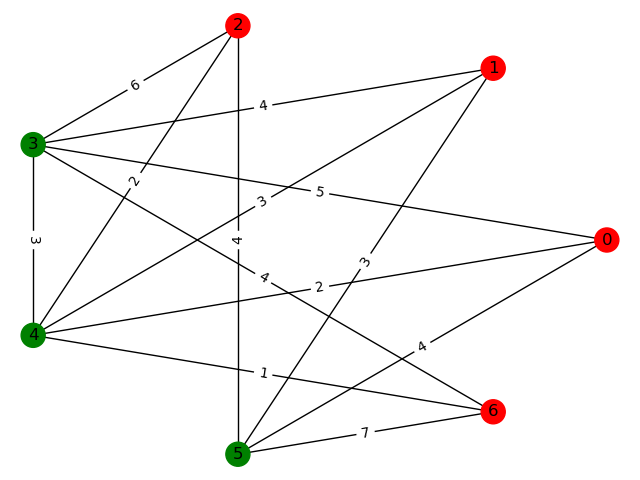
\includegraphics[width=0.49\linewidth]{pictures/new_network.png}
		\caption{Új hálózat}
		\label{routing-scheme}
	\end{center}
\end{figure}

\chapter{Teszt eredmények}

\section{Tesztelés menete}

A tesztelés során Erdős-Rényi gráfok voltak használva az egyszerű skálázhatóságból kifolyólag.
Három fő csoportba lehet a méréseket osztani a valószínűségi érték alapján, p = 0.25, p = 0.33 és p = 0.45.
A skálázhatóság tesztelésére különböző számú csúcspont volt használva, ezek rendre: 11, 15, 35, 50, 75, 100, 125, 150, 175 és 200.
A skálázhatósághoz még hozzátartozik a maximum fokszám, hogy mennyi gráf csúcs tud egyszerre kommunikálni, ezért az is meg van adva.
A valóságban van egy fizikai határ, hogy mennyi kliens tud csatlakozni egyszerre, ezért az értékek így lettek megválasztva, 3, 10, 16, 24 és 48.
A fenti paraméterek összes kombinációjára öt teszt lett futtat, majd azok átlagolva lettek.
Az adatok egy CSV fájlban lettek összegyűjtve, majd RapidMiner\cite{noauthor_lightning_nodate} segítségével lett kiértékelve.

\section{Átlag súlyozott úthossz}

\begin{figure}[h]
	\begin{center}
		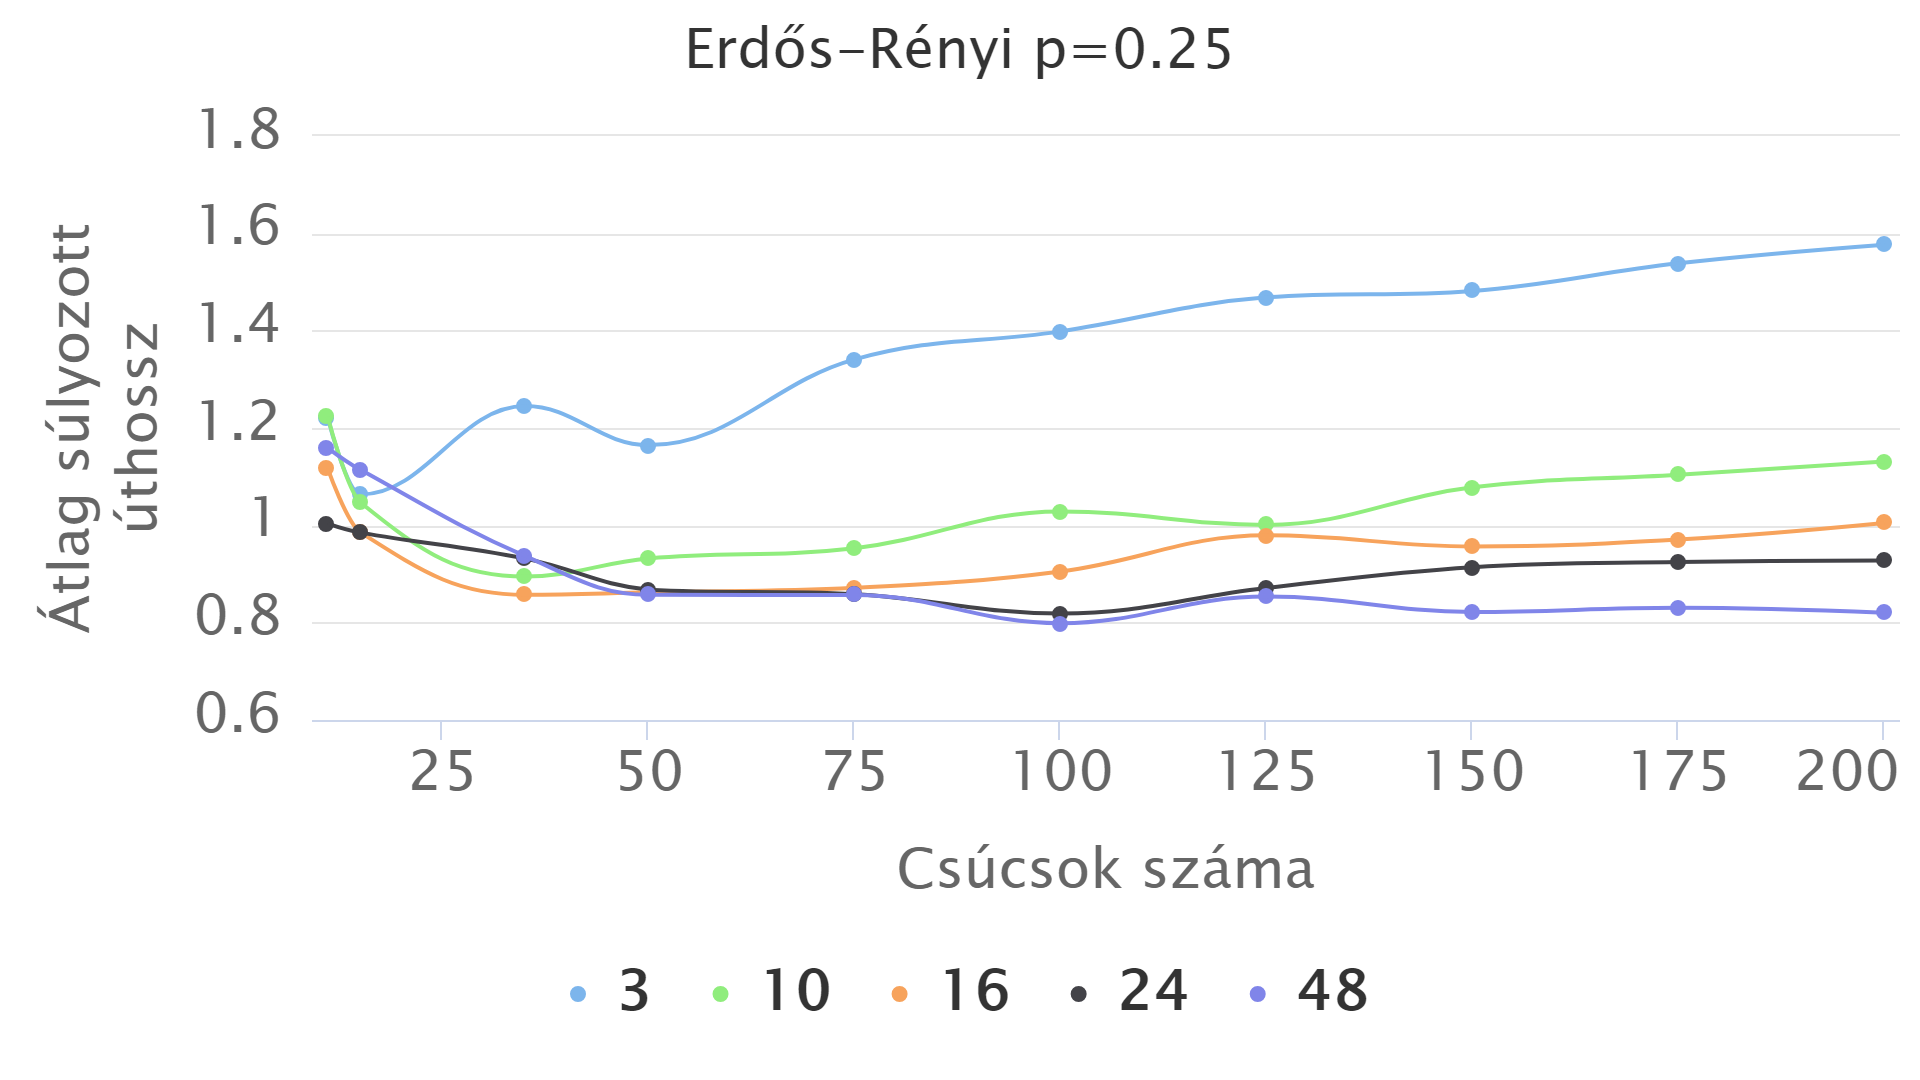
\includegraphics[width=0.40\linewidth]{pictures/constant_dan_ratio25_avg_route_len.png}
		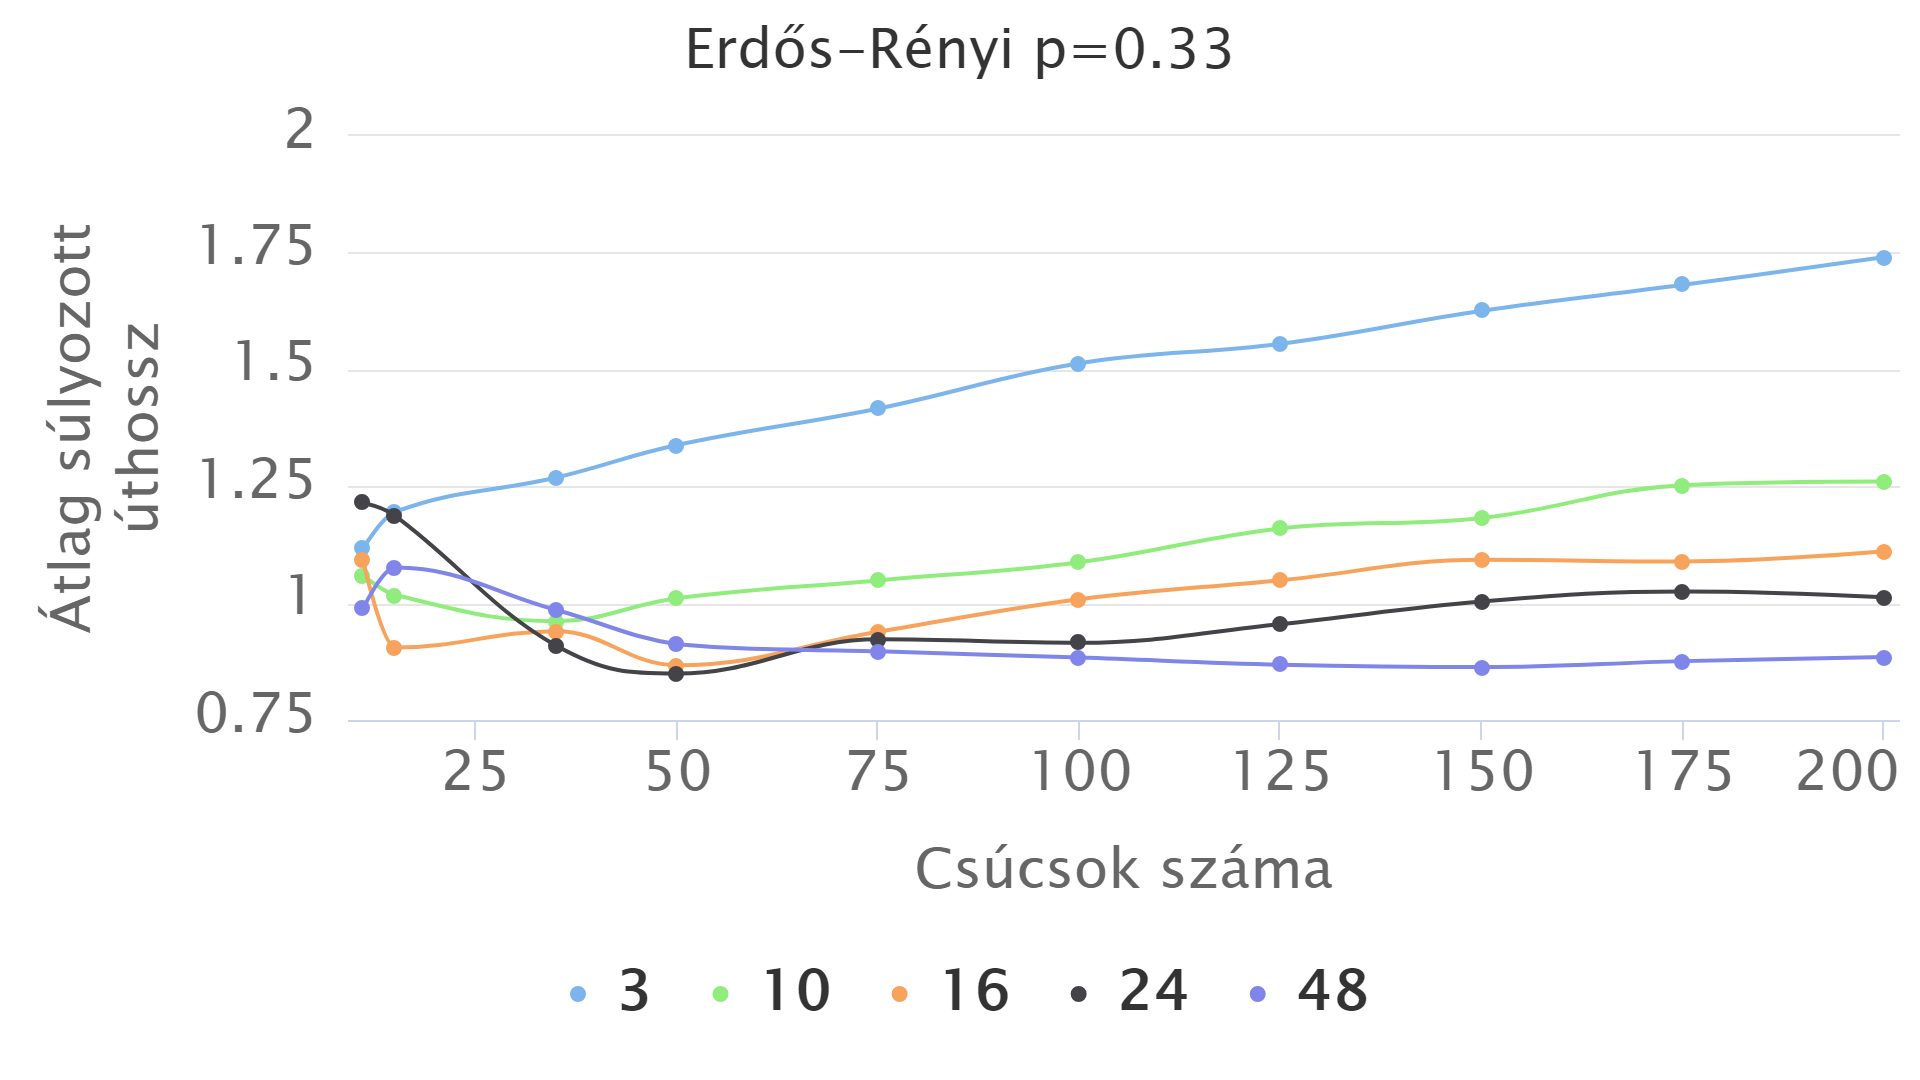
\includegraphics[width=0.40\linewidth]{pictures/constant_dan_ratio33_avg_route_len.png}
		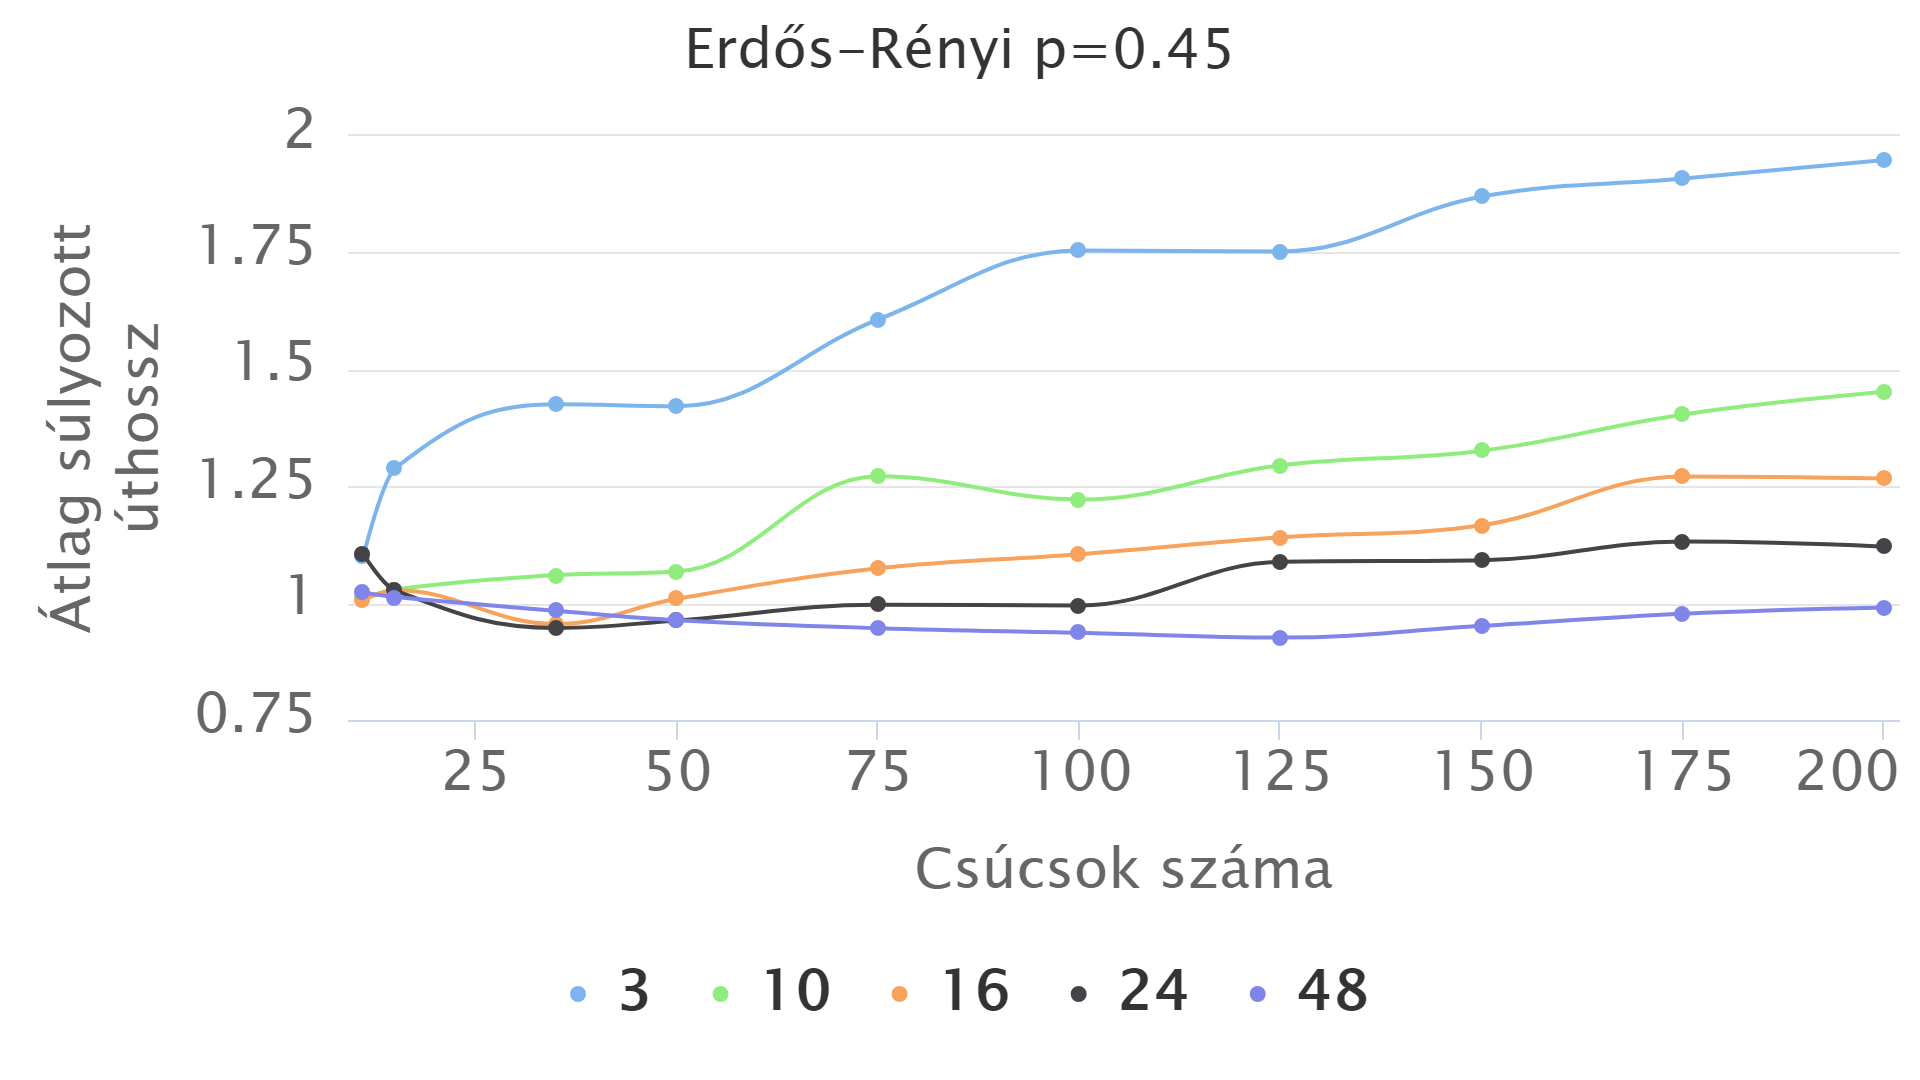
\includegraphics[width=0.40\linewidth]{pictures/constant_dan_ratio45_avg_route_len.png}
		\caption{Átlag súlyozott úthossz}
		\label{avg-len}
	\end{center}
\end{figure}


Az \ref{avg-len} ábrán látható az átlag súlyozott úthossz csúcspontok függvényében, és a delta fokszámra lebontva.
Az átlag súlyozott úthossz mind három esetben hasonlóan néz ki.
A konstans fokszám miatt egyértelműen látszik, hogy az értékek növekednek, kicsi delta esetén, pl. 3, ez nagyon jól megfigyelhető.
Az eredmények hasonlóak mind három esetben, a kitöltöttség növekedésével az értékek is növekednek, de a grafikon iránya nem változik.

\section{Átlag torlódás}

A \ref{congestion} ábrán látható az átlag torlódás. 
Hasonlóan mint az úthossznál a fő tényezők a csúcsok száma és az, hogy hogyan választjuk meg a fokszámot.
Ám ha megnézzük a két diagram irányát, két különböző dolgot mutatnak. 
A súlyozott úthossz növekedik ahogy hozzáveszünk további pontokat a hálózathoz, addig a torlódás mértéke közel exponenciálisan csökken.
Ennek egyszerű oka van, mert minél több csomópont közül tudunk választani, a terhelést egyre több pont között lehet elosztani és így a torlódás egészében csökken a hálózatban.

\begin{figure}[h]
	\begin{center}
		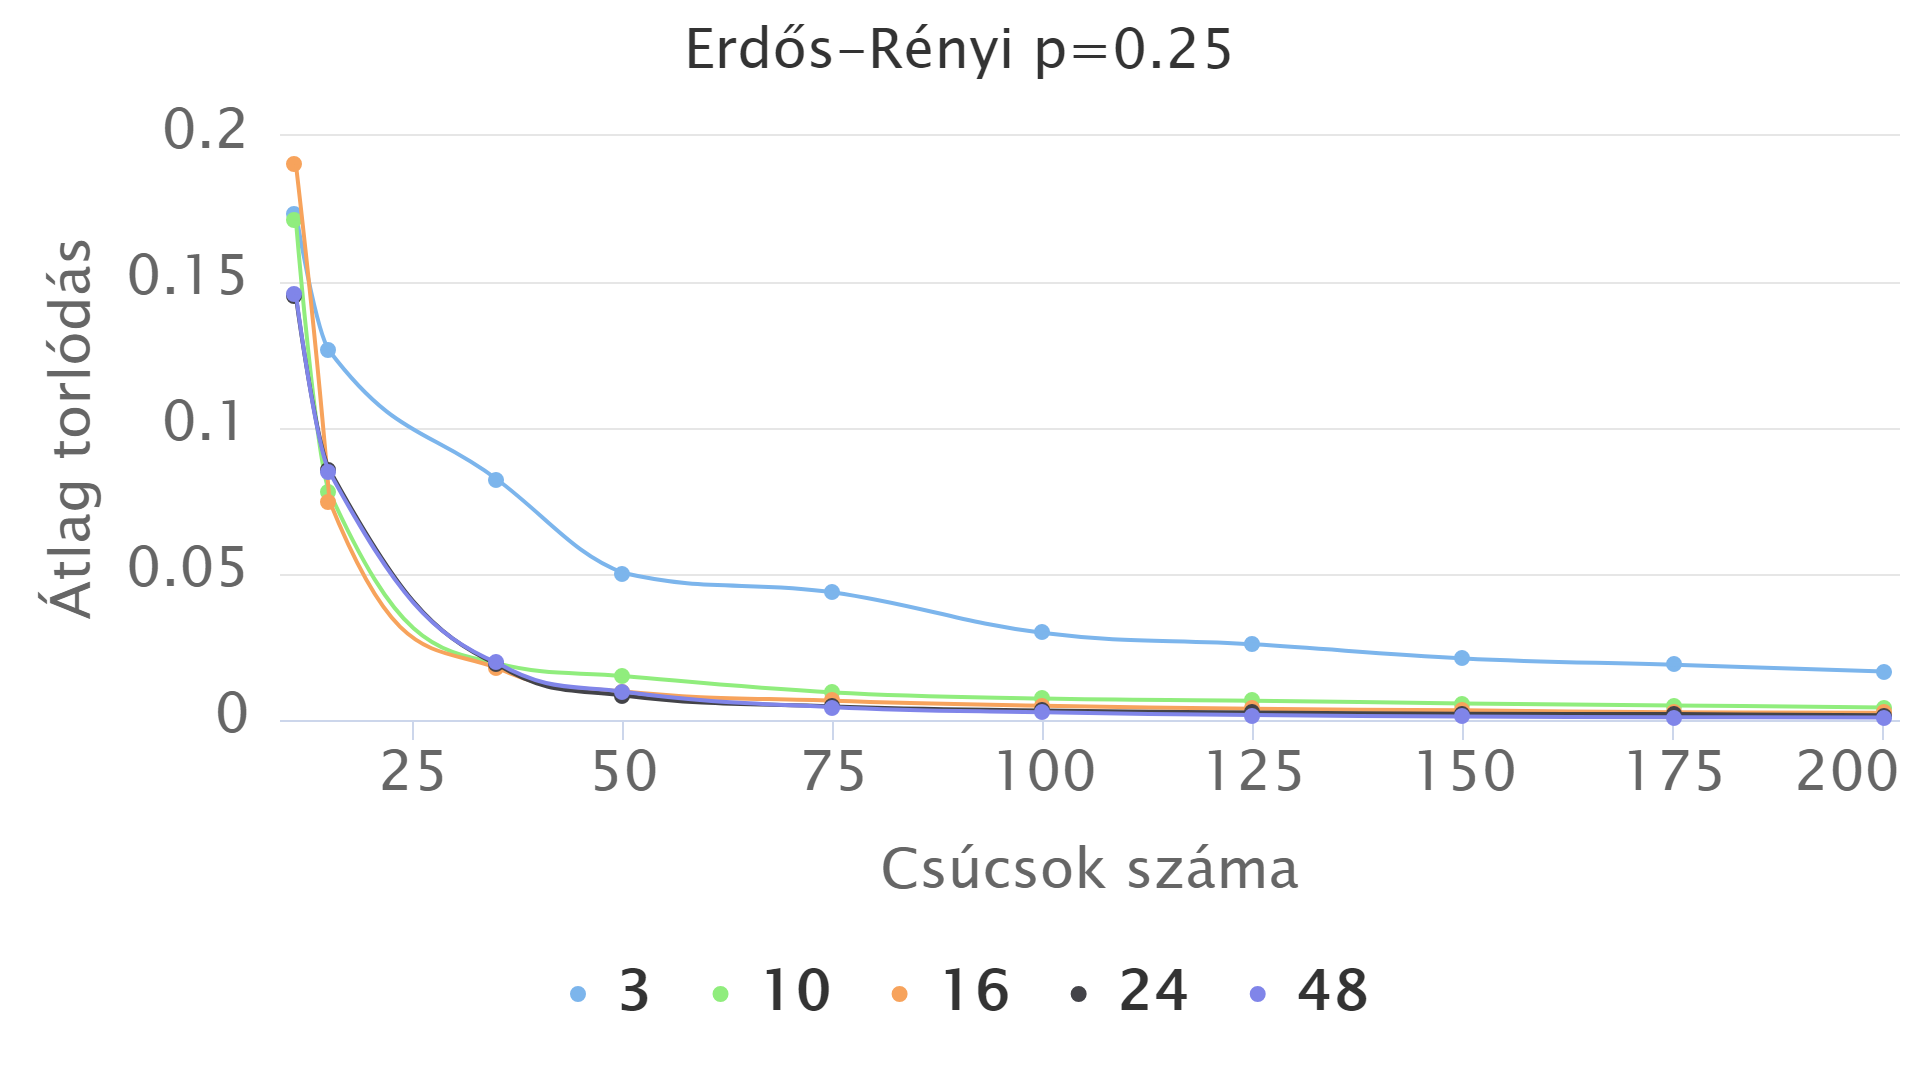
\includegraphics[width=0.40\linewidth]{pictures/constant_dan_ratio25_congestion.png}
		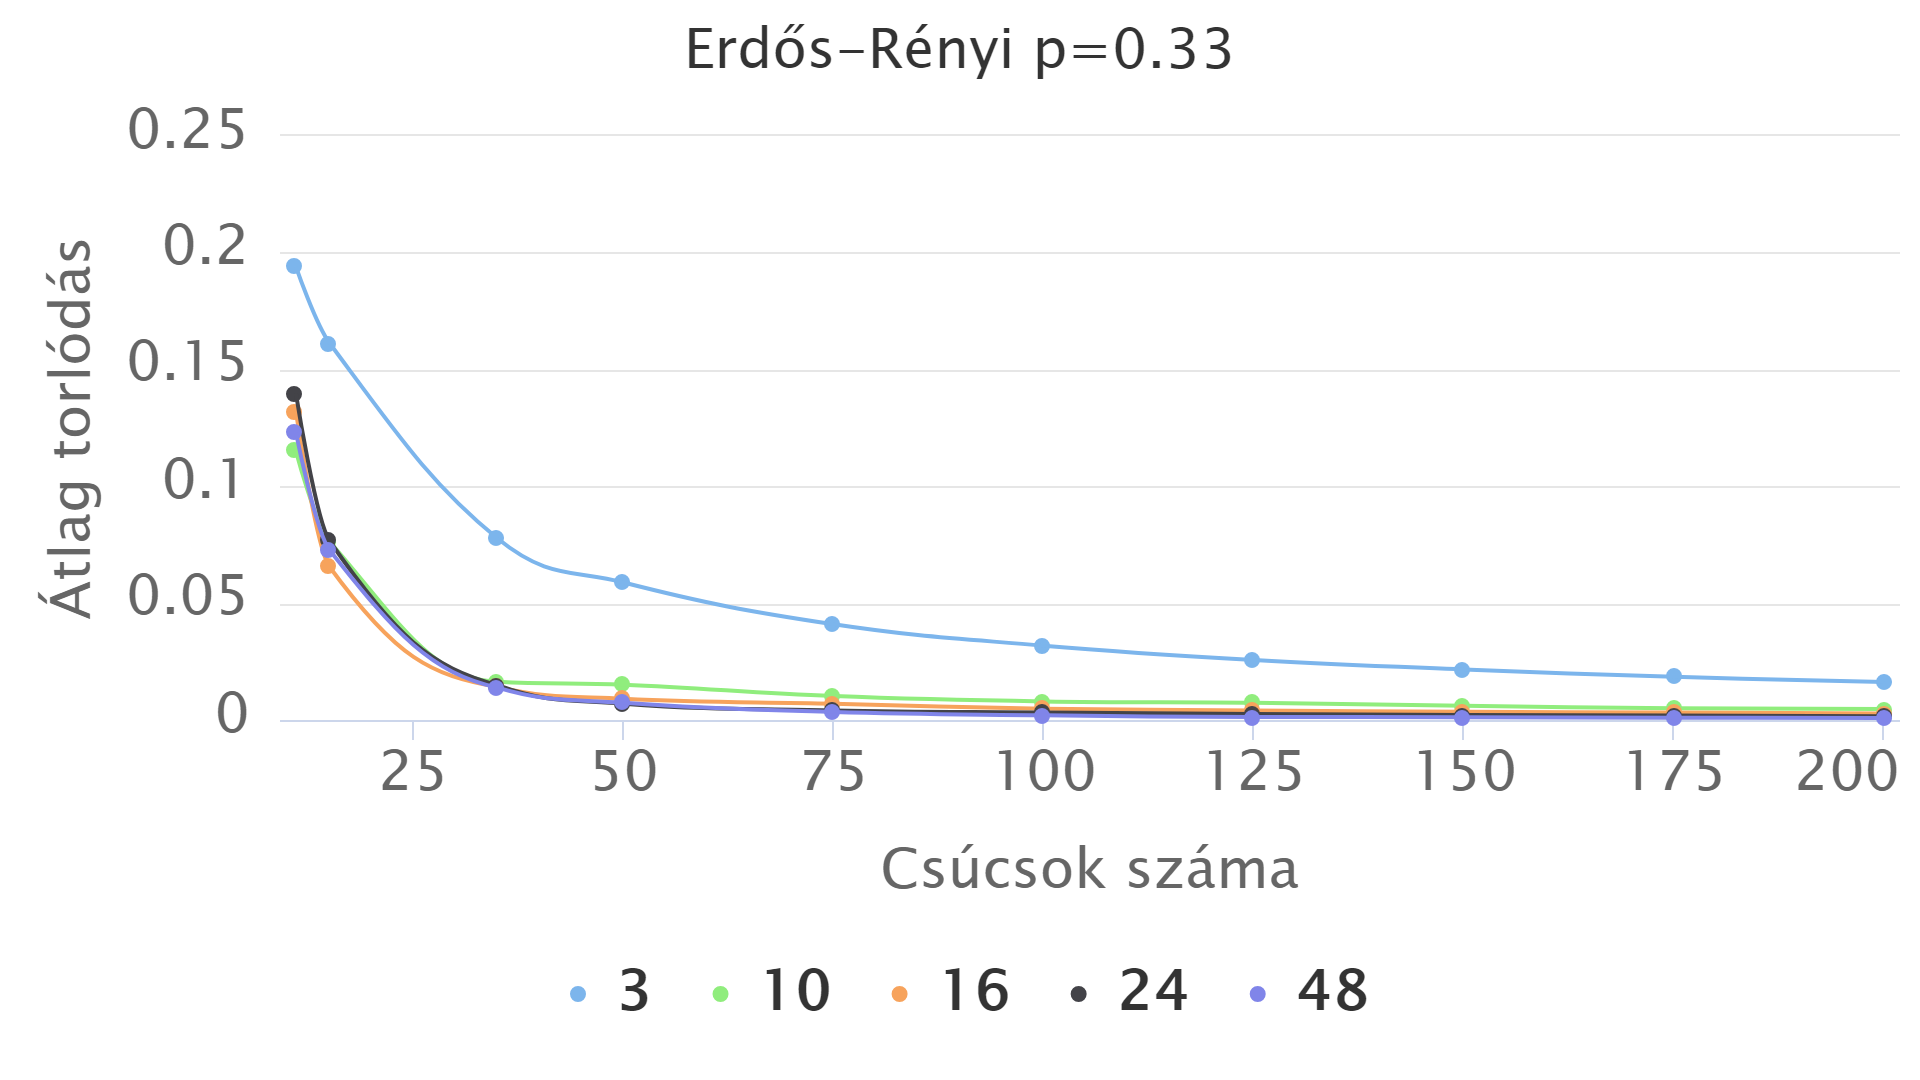
\includegraphics[width=0.40\linewidth]{pictures/constant_dan_ratio33_congestion.png}
		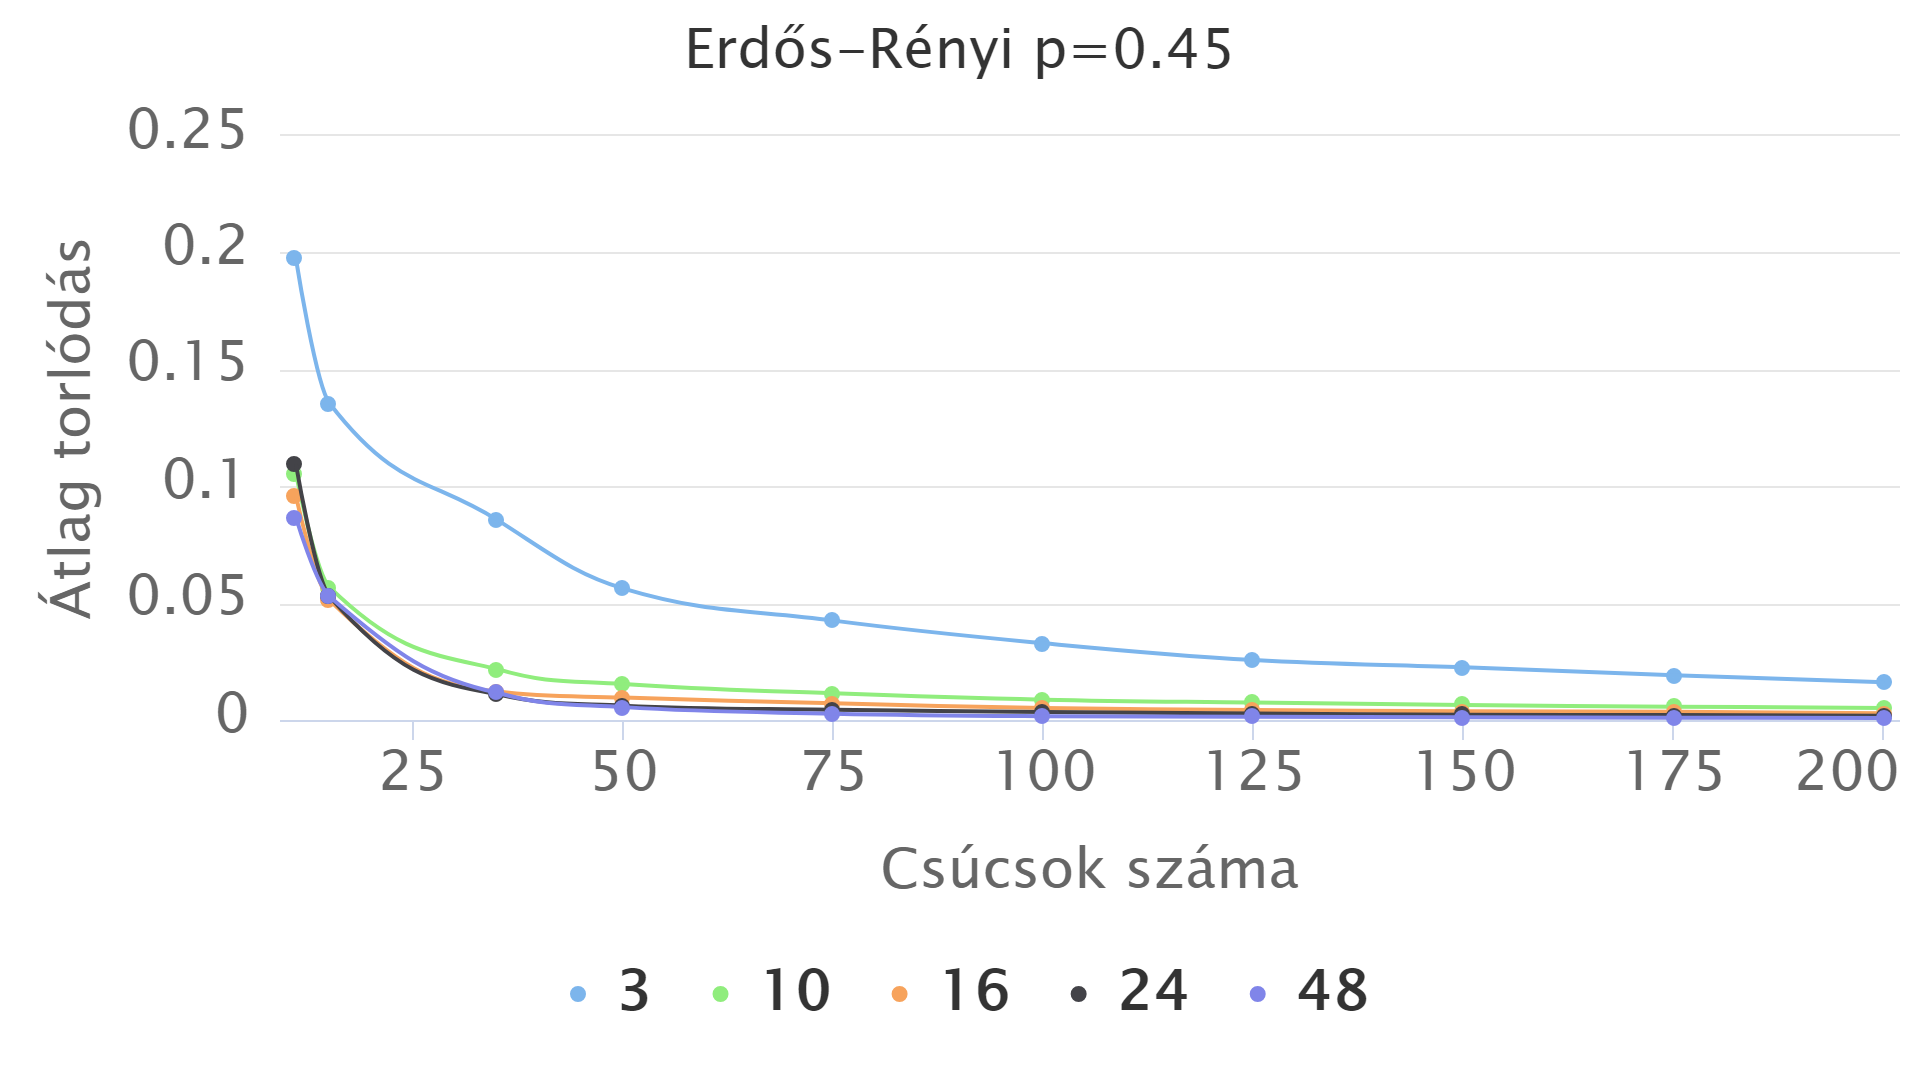
\includegraphics[width=0.40\linewidth]{pictures/constant_dan_ratio45_congestion.png}
		\caption{Átlag torlódás}
		\label{congestion}
	\end{center}
\end{figure}

\section{Fokszám}

A fentiekben már volt említve, hogy adott számú csomópontot használunk.
A cikkben szereplő felső korlátok az átlag fokszám függvényében van megadva, ami azt eredményezi, minden hálózatnak más $\Delta$ fokszám ad közel optimális megoldást.
Ez elméletben teljesül is, de ha megnézzük a \ref{delta} ábrát, rögtön észrevehető egy érdekes jelenség. 
A delta fokszám majdnem minden esetben nagyobb mint a csúcsok száma ami a hálózatban van.
Ez azt eredményezi, hogy minden csomópont közel két lépésből elérhető, és csak akkor van szükség az algoritmus újra rendező részére, 5. lépés, ha egy csomóponttal kommunikál több mint a fele pont a hálózatban.
Erre egy példa a 200 pontból álló hálózat, ami a képen látható, hogy már ha a $\Delta=4\rho$ a fokszámot annyi mint a pontok száma a hálózatban.

\begin{figure}[h]
	\begin{center}
		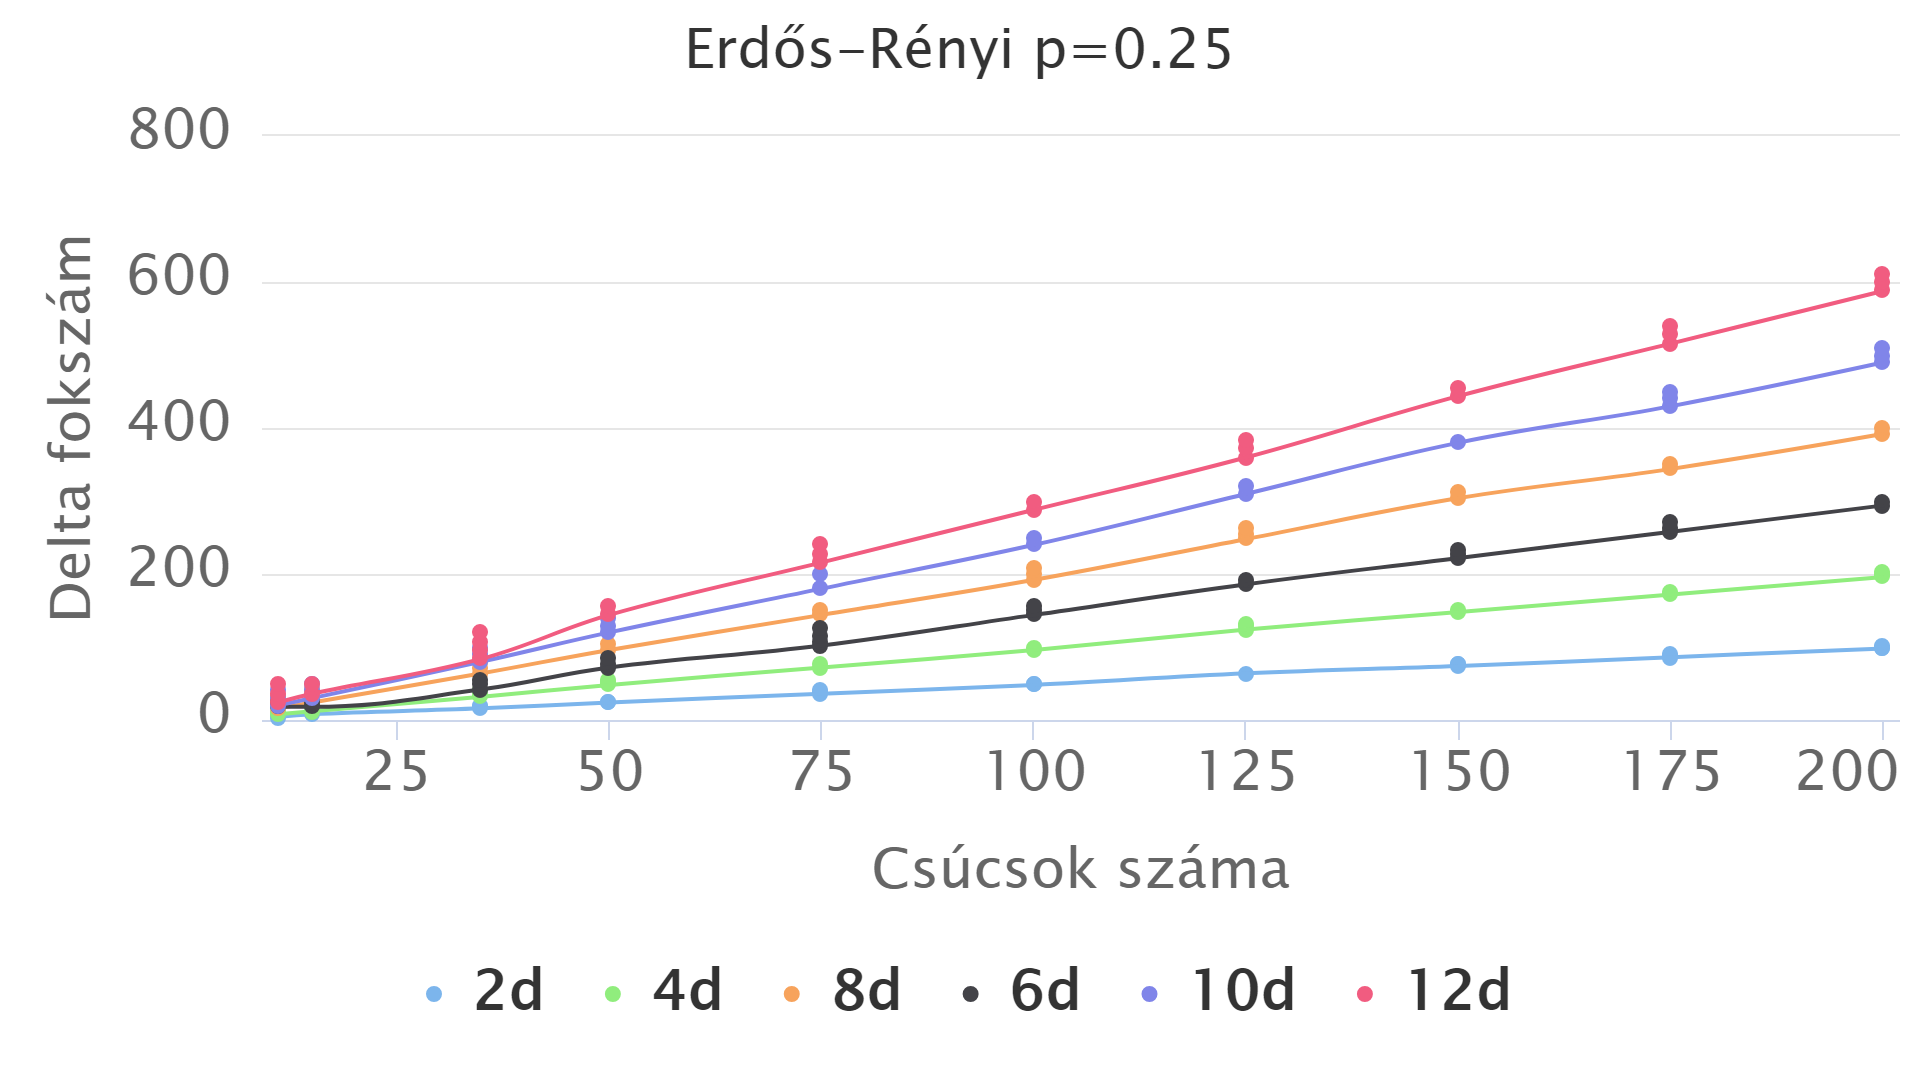
\includegraphics[width=0.40\linewidth]{pictures/constant_dan_ratio25_delta.png}
		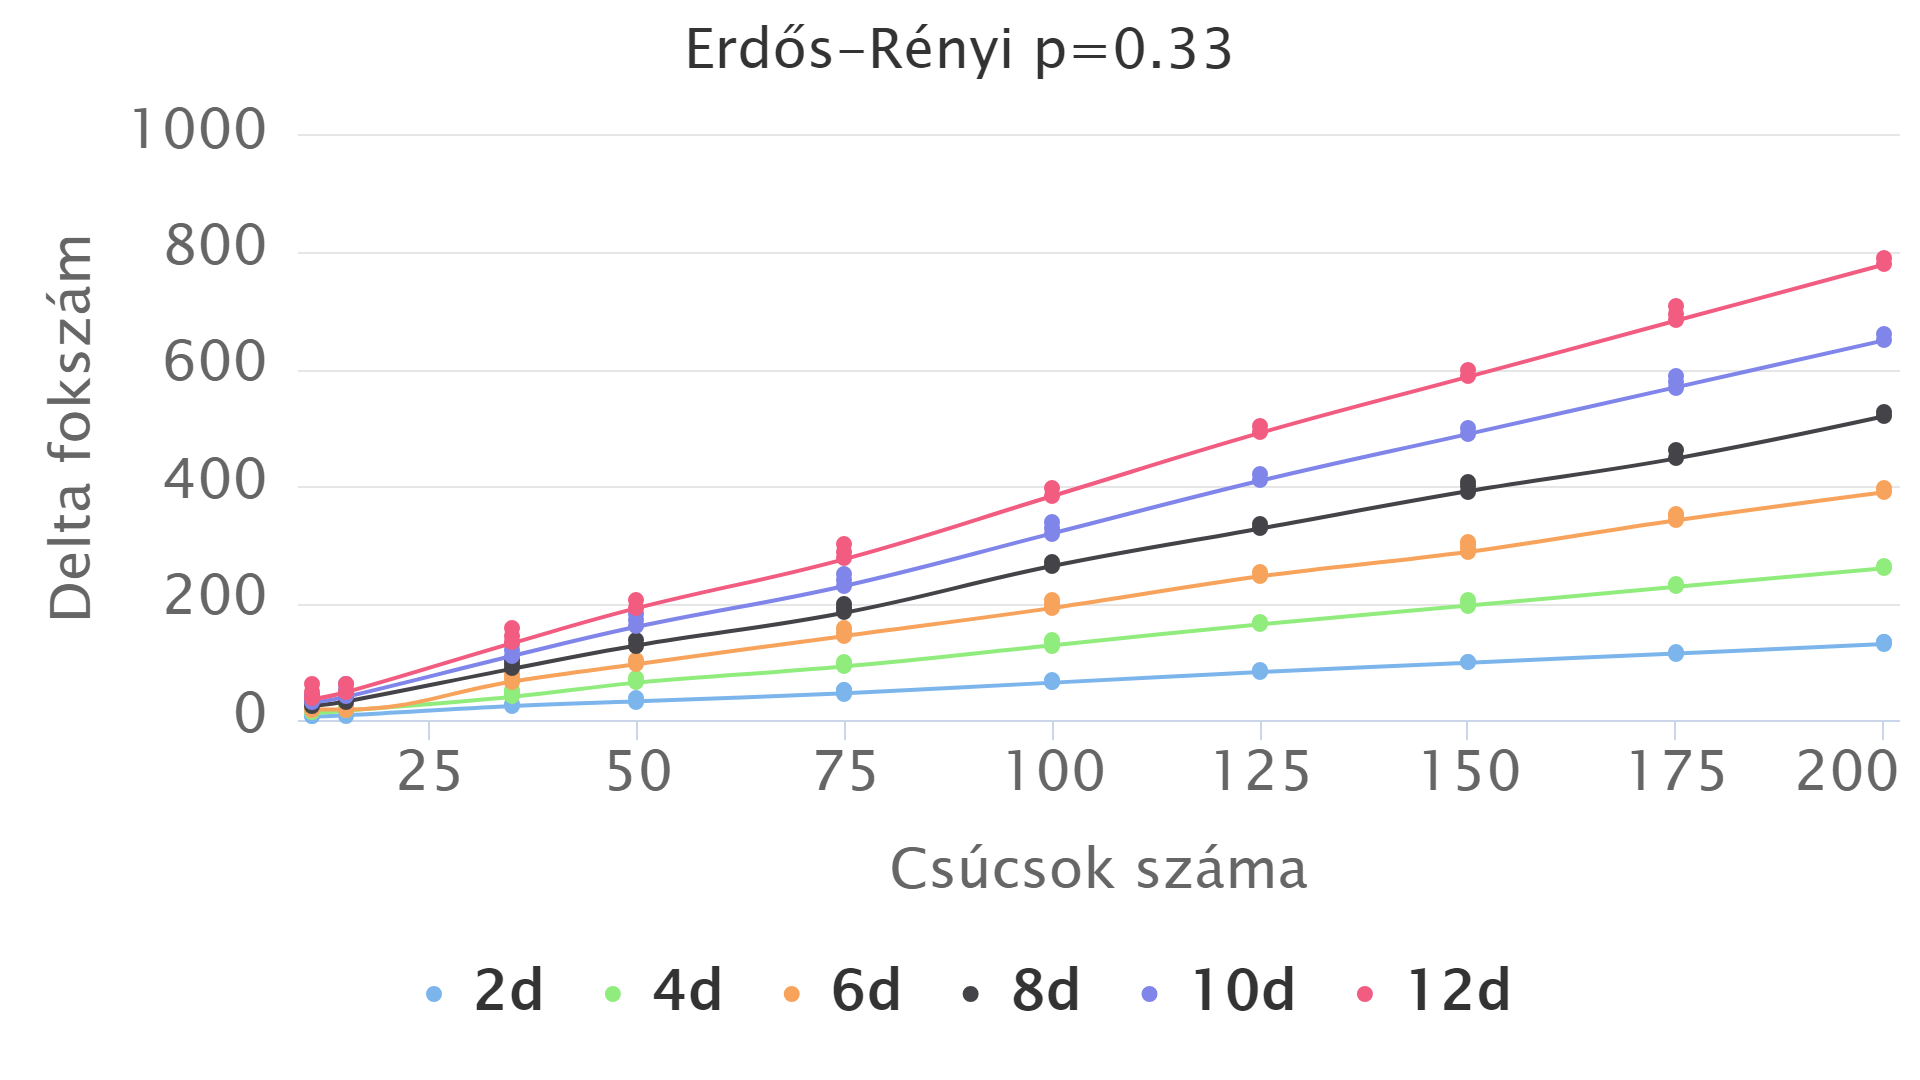
\includegraphics[width=0.40\linewidth]{pictures/constant_dan_ratio33_delta.png}		
		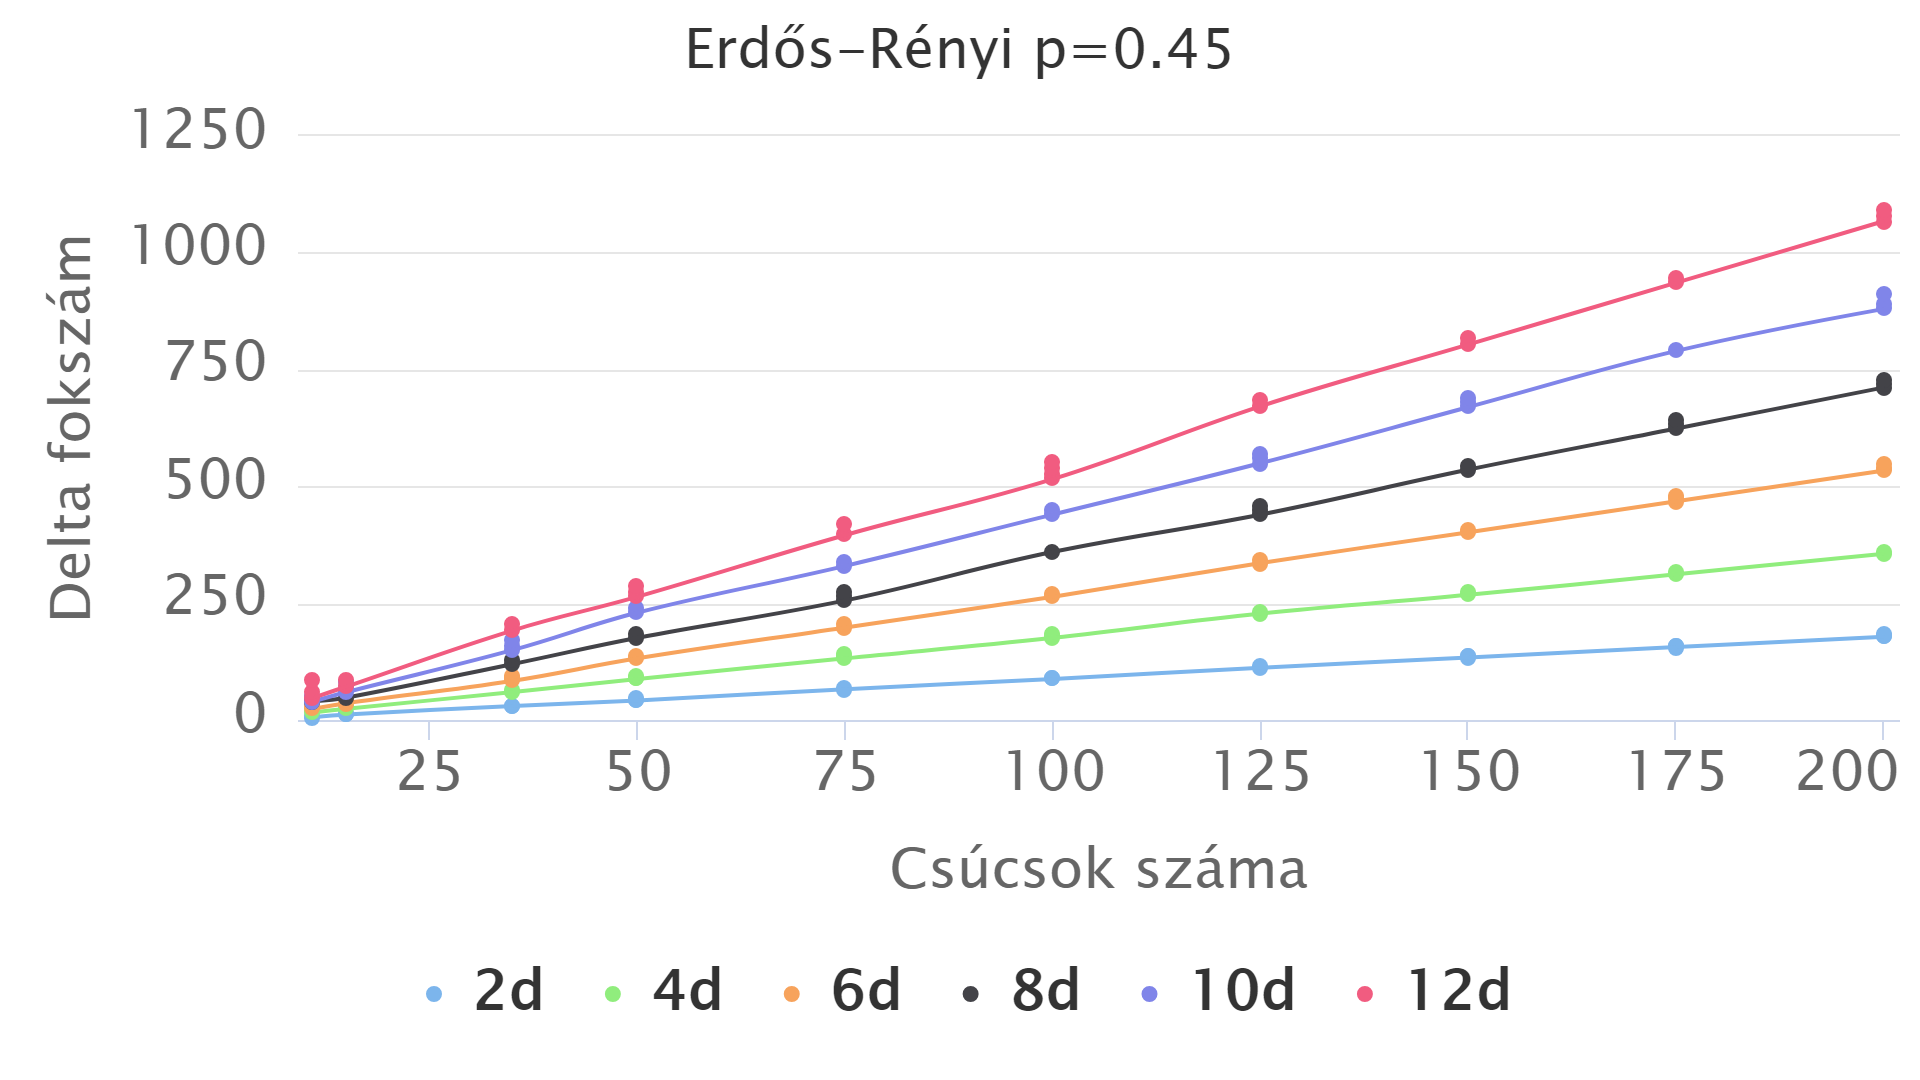
\includegraphics[width=0.40\linewidth]{pictures/constant_dan_ratio45_delta.png}
		\caption{Delta fokszám}
		\label{delta}
	\end{center}
\end{figure}

\chapter{Összefoglalás}

\section{Cikk eredménye}

Az technológia fejlődésével lehetőség nyílt arra, hogy a hálózatokat újrakonfiguráljuk futás időben.
A változó topológiának köszönhetően hatékonyabb lesz az adattárházak működése.
Az forgalom igény tudatos hálózatok tervezése körül jelenleg intenzív kutatás folyik ebből kifolyólag. 
A feldogozott cikk és a benne található algoritmus ad egy megoldást arra, hogy lehet ilyent tervezni.
Az algoritmus lényege, hogy a túlterhelt csomópontok között irányítsuk át forgalmat egy segéd csomóponton.
Ennek a megvalósítása az egófákkal van megadva, ahol lekorlátozzuk a maximális csatlakozások számát a jobban terhelt szerverekhez.
A szerzők által meghatároztak egy felső korlátot az átlag súlyozott úthosszra és torlódásra megadott fokszám mellett ami valóban megfelelő.


\section{Megjegyzések}

A teszt eredményekből látszik, hogy a $\Delta=12\rho$ fokszám egy nagyon magas korlát, mivel bőven túlmutat a rendelkezésre álló csúcsok számán. Feltételezhető, hogy ettől lehet jobb felső becslést is adni. 
Egy érdekes megfigyelés az algoritmus esetén, ha egy olyan fokszámot adunk meg, ami nem mutat túl a létező csúcspontok számán, hanem ellenkezőleg, elég szigorúra van véve.
Ilyenkor csak a magas fokszámú pontokra van garantálva, hogy a megadott fokszámú ponthoz csatlakoznak és ez nem fog teljesülni az alacsony fokszámúakra.
Egy ilyen eset legegyszerűbben akkor fordul elő, ha már telített a fokszáma a segítő pontnak magas fokú pontokkal. 
Mivel nem csak magas fokú csomópont fog kommunikálni egy segítővel, ezért még azokat is be kell húzni, mikor két segítő fog kommunikál, és ilyenkor nincs figyelve arra, hogy mi a jelenlegi fokszám. 

\bibliographystyle{abbrv}
\bibliography{refrences}

	
\end{document}